%%%%%%%%%%%%%%%%%%%%%%%%%%%%%%%%%%%%%%%%%%%%%%%%%%%%%%%%%%%%%%%%%%%%%%%%%%%%%%%%%%%%%%%%%%%%%%%%%%%%

\chapter{Details on The Molecular ISM in the SSCs in \ngc253}
\chaptermark{Details on the SSC ISM}
\label{appendix: SSCs}

%%%%%%%%%%%%%%%%%%%%%%%%%%%%%%%%%%%%%%%%%%%%%%%%%%%%%%%%%%%%%%%%%%%%%%%%%%%%%%%%%%%%%%%%%%%%%%%%%%%%

\section{Details of \xclass fitting}
\label{appendix: SSCs: xclass}

\subsection{Handling of blended lines in the first fit run}
Joint fitting of multiple species with insufficient constraints increases the number of degrees of freedom to a point where the fitter does not converge reliably anymore. 
We therefore fit the species listed in Table~\ref{SSCs: table: intensities} independently where possible or include potential blended lines in the fit if necessary. 
For CO, CS, HCN, HCO+, H2CS, H$^{13}$CN, HC$^{15}$N, H$^{15}$NC, SO, $^{33}$SO, SO$_2$ and HCN ($\nu_2=1$) completely independent fitting is possible with appropriately selected fit range. The other species HCN ($\nu_2=2$'), H$C_3$N ($\nu=0$'),
H$C_3$N ($\nu_6=1$'), H$C_3$N ($\nu_6=2$'), H$C_3$N ($\nu_7=1$'), H$C_3$N ($\nu_7=2$'), $^{34}$SO ($\nu=0$'), S$^{18}$O ($\nu=0$') and $^{34}$SO2 ($\nu=0$') must be fitted jointly with lines of other species.

\subsection{\xclass fit parameters}
\xclass models the spectra based on the molecular parameters of the species to be fitted and can directly solve for physical quantities such as rotational (vibrational) temperature and column density. Further fit parameters are linewidth and centroid of the line. As we work with single pixel spectra, we leave the additional \emph{source size parameter} fixed at unity. This assumes the source to completely fill the beam ($0.13\arcsec \times 0.17\arcsec$, $\sim 2.5$\,pc) as is indicated by the SSC sizes of $\sim 1.5-4$\,pc obtained by \Leroy{t}.

\xclass allows to fit for \emph{excitation temperature} even when only one line of a species is detected due to the effect on the line shape (e.g. flattening due to opacity). 
However, with a single transition the temperature cannot be well constrained and the results scatter wildly. The fitted excitation temperature in such a case strongly depends on the line shape that is easily influenced by random noise fluctuations.
For the species with only a single line detected, we therefore need to fix the temperature. In the case of multiple detected lines (SO$_2$, H$_2$CS), the temperature also scatters considerably and sometimes even provides unphysical results (e.g. higher than the molecular binding energy) when the fit fails to converge successfully. Hence, we fix the rotational temperature $\mathrm{T_{rot}} = 130$\,K which is the temperature of the warm ISM component found by \citet{2013ApJ...779...33M} and \citet{Gorski:2017es} at lower spatial resolution. Assuming this temperature keeps our analysis consistent with \Leroy{t} who also assumed 130\,K. The observed CO peak brightness temperature $\mathrm{T_b} = 60-130$\,K may act as a proxy for $\mathrm{T_{rot}}$ under certain assumptions (optically thick emission, beam filling factor unity). Since we measure $\mathrm{T_{rot}} \sim 130$\,K (Section~\ref{SSCs: section: ISM temperature}), one of these assumptions is not met. The excitation temperature $\mathrm{T_{vib}}$ of vibrationally excited species is certainly higher but difficult to estimate. Line ratios of vibrational states with differing $\mathrm{E_{upper}}$ (or $\mathrm{E_{lower}}$) could place limits on $\mathrm{T_{vib}}$ but in many SSCs no vibrationally excited species are detected. We therefore use a common fixed excitation temperature of $\mathrm{T_{vib}} = 300$\,K. This value is supposedly on the lower side of the actual excitation temperatures and thus causes the column densities of the vibrationally excited states to be on the higher side. The observed emission intensity is influenced by temperature and column density because higher excitation and more emitting molecules provide stronger line emission. In SO$_2$, the most reliable temperature tracer in our sample, changes in temperature and column density are inversely correlated at ratios of $0.8-1.0$ in the SSCs with successful temperature estimation (cf. Section~\ref{SSCs: section: ISM temperature}). This means any under-/overestimation of the fixed temperatures by a factor $x$ directly translate to an $x$ times under-/overestimation in column density. A factor of 2 variation in the chosen excitation temperature ($65\,\mathrm{K} \LESS \mathrm{T_{rot}} \LESS 260\,\mathrm{K}$ and $150\,\mathrm{K} \LESS \mathrm{T_{vib}} \LESS 600\,\mathrm{K}$) is well plausible in the SSCs. Hence, the derived column densities should be understood with a systematic error of a factor of two.

We apply loose limits on column density ($10^{12} - 10^{25}$\,\pcm2), linewidth ($5-80$\,\kms) and line centroid ($-10 - 10$\,\kms relative to the first manual estimate in Section~\ref{SSCs: section: spectra}). For the second run these are limited to the $16^\mathrm{th} - 84^\mathrm{th}$ percentile ranges of the first run.

\subsection{Fit algorithm}
\xclass offers a choice of algorithms that can be daisychained to allow for faster and more robust exploration of the parameter space depending on the dataset. For this dataset, the fitting generally works well and is robust against repetition of the fit and variations of the initial guesses. For some species in a few SSCs, it is necessary to adjust initial guesses or boundaries of the fit parameters to allow the algorithm to find a solution.
We use a combination of two algorithms in sequence to assure the solver finds the global minimum of the fit and then converges to this minimum. We achieve this by a combination of 50 iterations of the ``Genetic'' algorithm followed by 50 iterations of the ``Levenberg-Marquardt'' algorithm. For a detailed description of the fit algorithms, we refer to \citep{2018ascl.soft10016M}.

\subsection{Error estimation}
This \xclass fitting procedure reliably finds the best fit but does not estimate errors of the fit parameters. We therefore bootstrap the errors using a Monte-Carlo scheme: We draw 100 versions of Gaussian noise and add it to the observed spectra which are then fitted as described above. The added Gaussian noise is set up with standard deviation 0.46\,K, the measured RMS noise in the data. This scheme tests the robustness of the fit to noise fluctuations in the data and thus the statistical error of the fit. Systematic errors such as the flux uncertainty of $\LESSSIM5$\% for ALMA observations (ALMA Technical Handbook) apply additionally. Of the 100 fit variations plus a fit to the unaltered spectra, we report the median and $16^\mathrm{th}$ to $84^\mathrm{th}$ percentiles range\footnote{The range $16^\mathrm{th}$ to $84^\mathrm{th}$ percentiles corresponds to $-1\sigma$ to $+1\sigma$ for Gaussian distributions.} as best estimate and respective error margin for each parameter.


%%%%%%%%%%%%%%%%%%%%%%%%%%%%%%%%%%%%%%%%%%%%%%%%%%%%%%%%%%%%%%%%%%%%%%%%%%%%%%%%%%%%%%%%%%%%%%%%%%%%

\section{SSC energy source using line intensity ratios}
\label{appendix: SSCs: energy source intensity}

As discussed in Section~\ref{SSCs: section: energy source}, the model by \citet{Loenen:2008fb} and \citet{Baan:2008hx} provides a tool to estimate the excitation environment in the SSCs which can then be interpreted for the potential energy sources.
Since we derive column densities with XCLASS, we can directly use physical quantities for this analysis instead of observational quantities. As a test, however, we also construct the ratio diagrams for line ratios in Figure~\ref{SSCs: figure: XDR PDR intensity}. Note that in this case the correction of the observed H$^{15}$NC to H$^{14}$NC is only an approximation because we do not consider optical depth but only the observed line intensity ratios.
Nonetheless, we arrive at the same conclusion that the chemistry in the SSCs is powered by PDRs rather than XDRs. The exact placement in the ratio--ratio planes is slightly different, though, with deviations of $\sim 0.1-0.2$\,dex. SSCs~2 and 3 are not compatible with XDR conditions which was barely the case for the column density ratios (Figure~\ref{SSCs: figure: XDR PDR column densities}).

The density estimation deviates between estimation from line ratios and column density ratios. The CS/HCN line ratios are consistently $\LESS 1$ suggesting $N_H \LESS 10^{22}$\,\pcm2. This is in tension with the fact that the SSCs are undetected at IR wavelength and thus must be hidden behind large columns of dust.
The assumption that column density ratios can be approximated by line ratios \citep[as done in e.g.][]{Baan:2008hx} is not valid, at least in the case of NGC~253's SSCs.

As in Section~\ref{SSCs: section: energy source}, we overplot the measurement from \citet[central 440\,pc]{Baan:2008hx} and the 10 selected regions from \citet[][40\,pc]{2015ApJ...801...63M}. As opposed to the column density ratios (Figure~\ref{SSCs: figure: XDR PDR column densities}, the large scale measurement of \citet{Baan:2008hx} deviates from the SSCs towards higher HNC/HCO$^+$ and slightly lower HCO$^+$/HCN but is still close to the ratios in SSCs~2 and 3. Arguably, this is caused by the large amount of molecular gas outside the SSCs that we focus on.
The regions by \citep{2015ApJ...801...63M} are consistent with our measurements in HNC/HCN vs. HNC/HCO$^+$ but are offset towards lower HCO$^+$/HCN by $\sim 0.1$ as seen in the upper two panels. This is most likely a systematic effects in the measured HCN or HCO$^+$ intensities.

\begin{figure*}
    \centering
    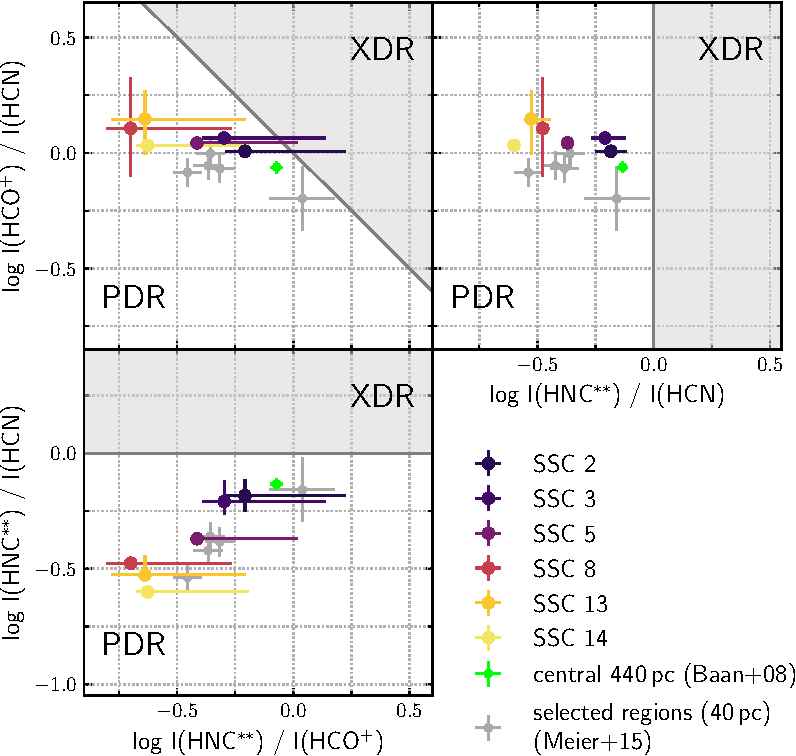
\includegraphics[width=0.58\linewidth]{images/chapters/papers/SSCs/SSCs_XDR-PDR_integrated_intensity.pdf}
    \caption[PDR--XDR chart based on line intensities]{PDR--XDR chart according to \citet{Loenen:2008fb} and \citet{Baan:2008hx} for ratios of HCN, HCO$^+$ and HNC intensities. In our observations, we do not observe H$^{14}$NC but H$^{15}$NC which we estimate using the isotope ratio $^{14}$N/$^{15}$N from H$^{14}$NC and H$^{15}$NC. In the plots, this is marked by $^{**}$ in the labels. The correction is possible for only 6 out of 14 SSCs due to the detection rate of H$^{15}$NC. The \citet{Baan:2008hx} estimate for the central region of NGC~253 extends over all SSCs and surrounding gas.
    }
    \label{SSCs: figure: XDR PDR intensity}
\end{figure*}